\chapter{Reporting}

\noindent
One important part of SDR is the way we gather and aggregate all recorded data
from all our systems and finally compile simple reports. One major goal, when
designing the reporting module, was to be able to get all these things in
matter of minutes, saving your time in front of computer. As well, another 
important part was to be able to use different data visualization engines 
for all recorded data.

\section{Design}
By default, the reportign package uses RRDtool, the high performance data logging 
and graphing system as our performance database. We generate all reports, plots 
based on RRDtool.

However we are not restricted to RRDtool since we do have all raw data collected. 
We are using as well R statistical computing and graphics language for analysing 
all recorded data using heatmaps or treemaps representation. At last, we like 
to bring closely geometry and performance analysis: cuplayer, a visual player 
of multiprocessor data, cpurec, using Barycentric coordinates, which displays 
the CPU transition states from IDLE to USER or SYSTEM time.

\begin{figure}[!ht]
\centering
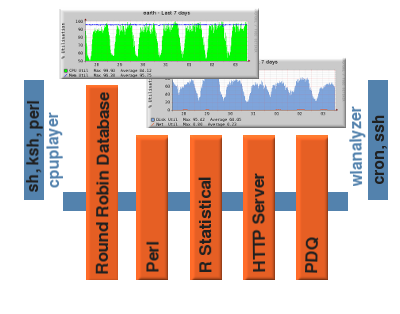
\includegraphics[width=75mm,height=55mm]{sdr-rep-schemaf.png}
\caption{SDR Reporting module}
\label{fig:sdr-rep-schemaf}
\end{figure}

This way, SDR Reporting contains several sub-modules, each with its own purpose:

\begin{enumerate}

\item Data visualization engine:\\
a standard component responsible for all plots and reports within SDR Reporting. 
This uses RRDtool, R, cpuplayer and Perl

\item Workload management engine:\\
includes different workload management tools for web and streaming based 
services: 
\begin{itemize}
 \item wlanalyzer: HTTP based workloads
 \item slanalyzer: RTMP, RTSP based workloads
\end{itemize}

\end{enumerate}

All these things make the reporting module simple and apart from other 
reporting systems:

\begin{itemize}
\item Not an analytics package
\item Simple pre-compiled reports, always work
\item Very simple to understand
\item Easy customizations
\item You don't have to click, dozens of options, links to get what you need
\item Should save your time in front of computer, being simple and to the point
\item Simple to educate your IT staff
\end{itemize}

\section{Configuration}


\endinput
